\documentclass[12pt]{letter}\usepackage[letterpaper,margin=0.65in]{geometry}\usepackage{textcomp}\usepackage{graphicx}\usepackage[rflt]{floatflt}\pagenumbering{gobble}\begin{document}\begin{floatingfigure}{0.15\textwidth}\raisebox{0pt}[0pt][0pt]{\raisebox{-2.5cm}{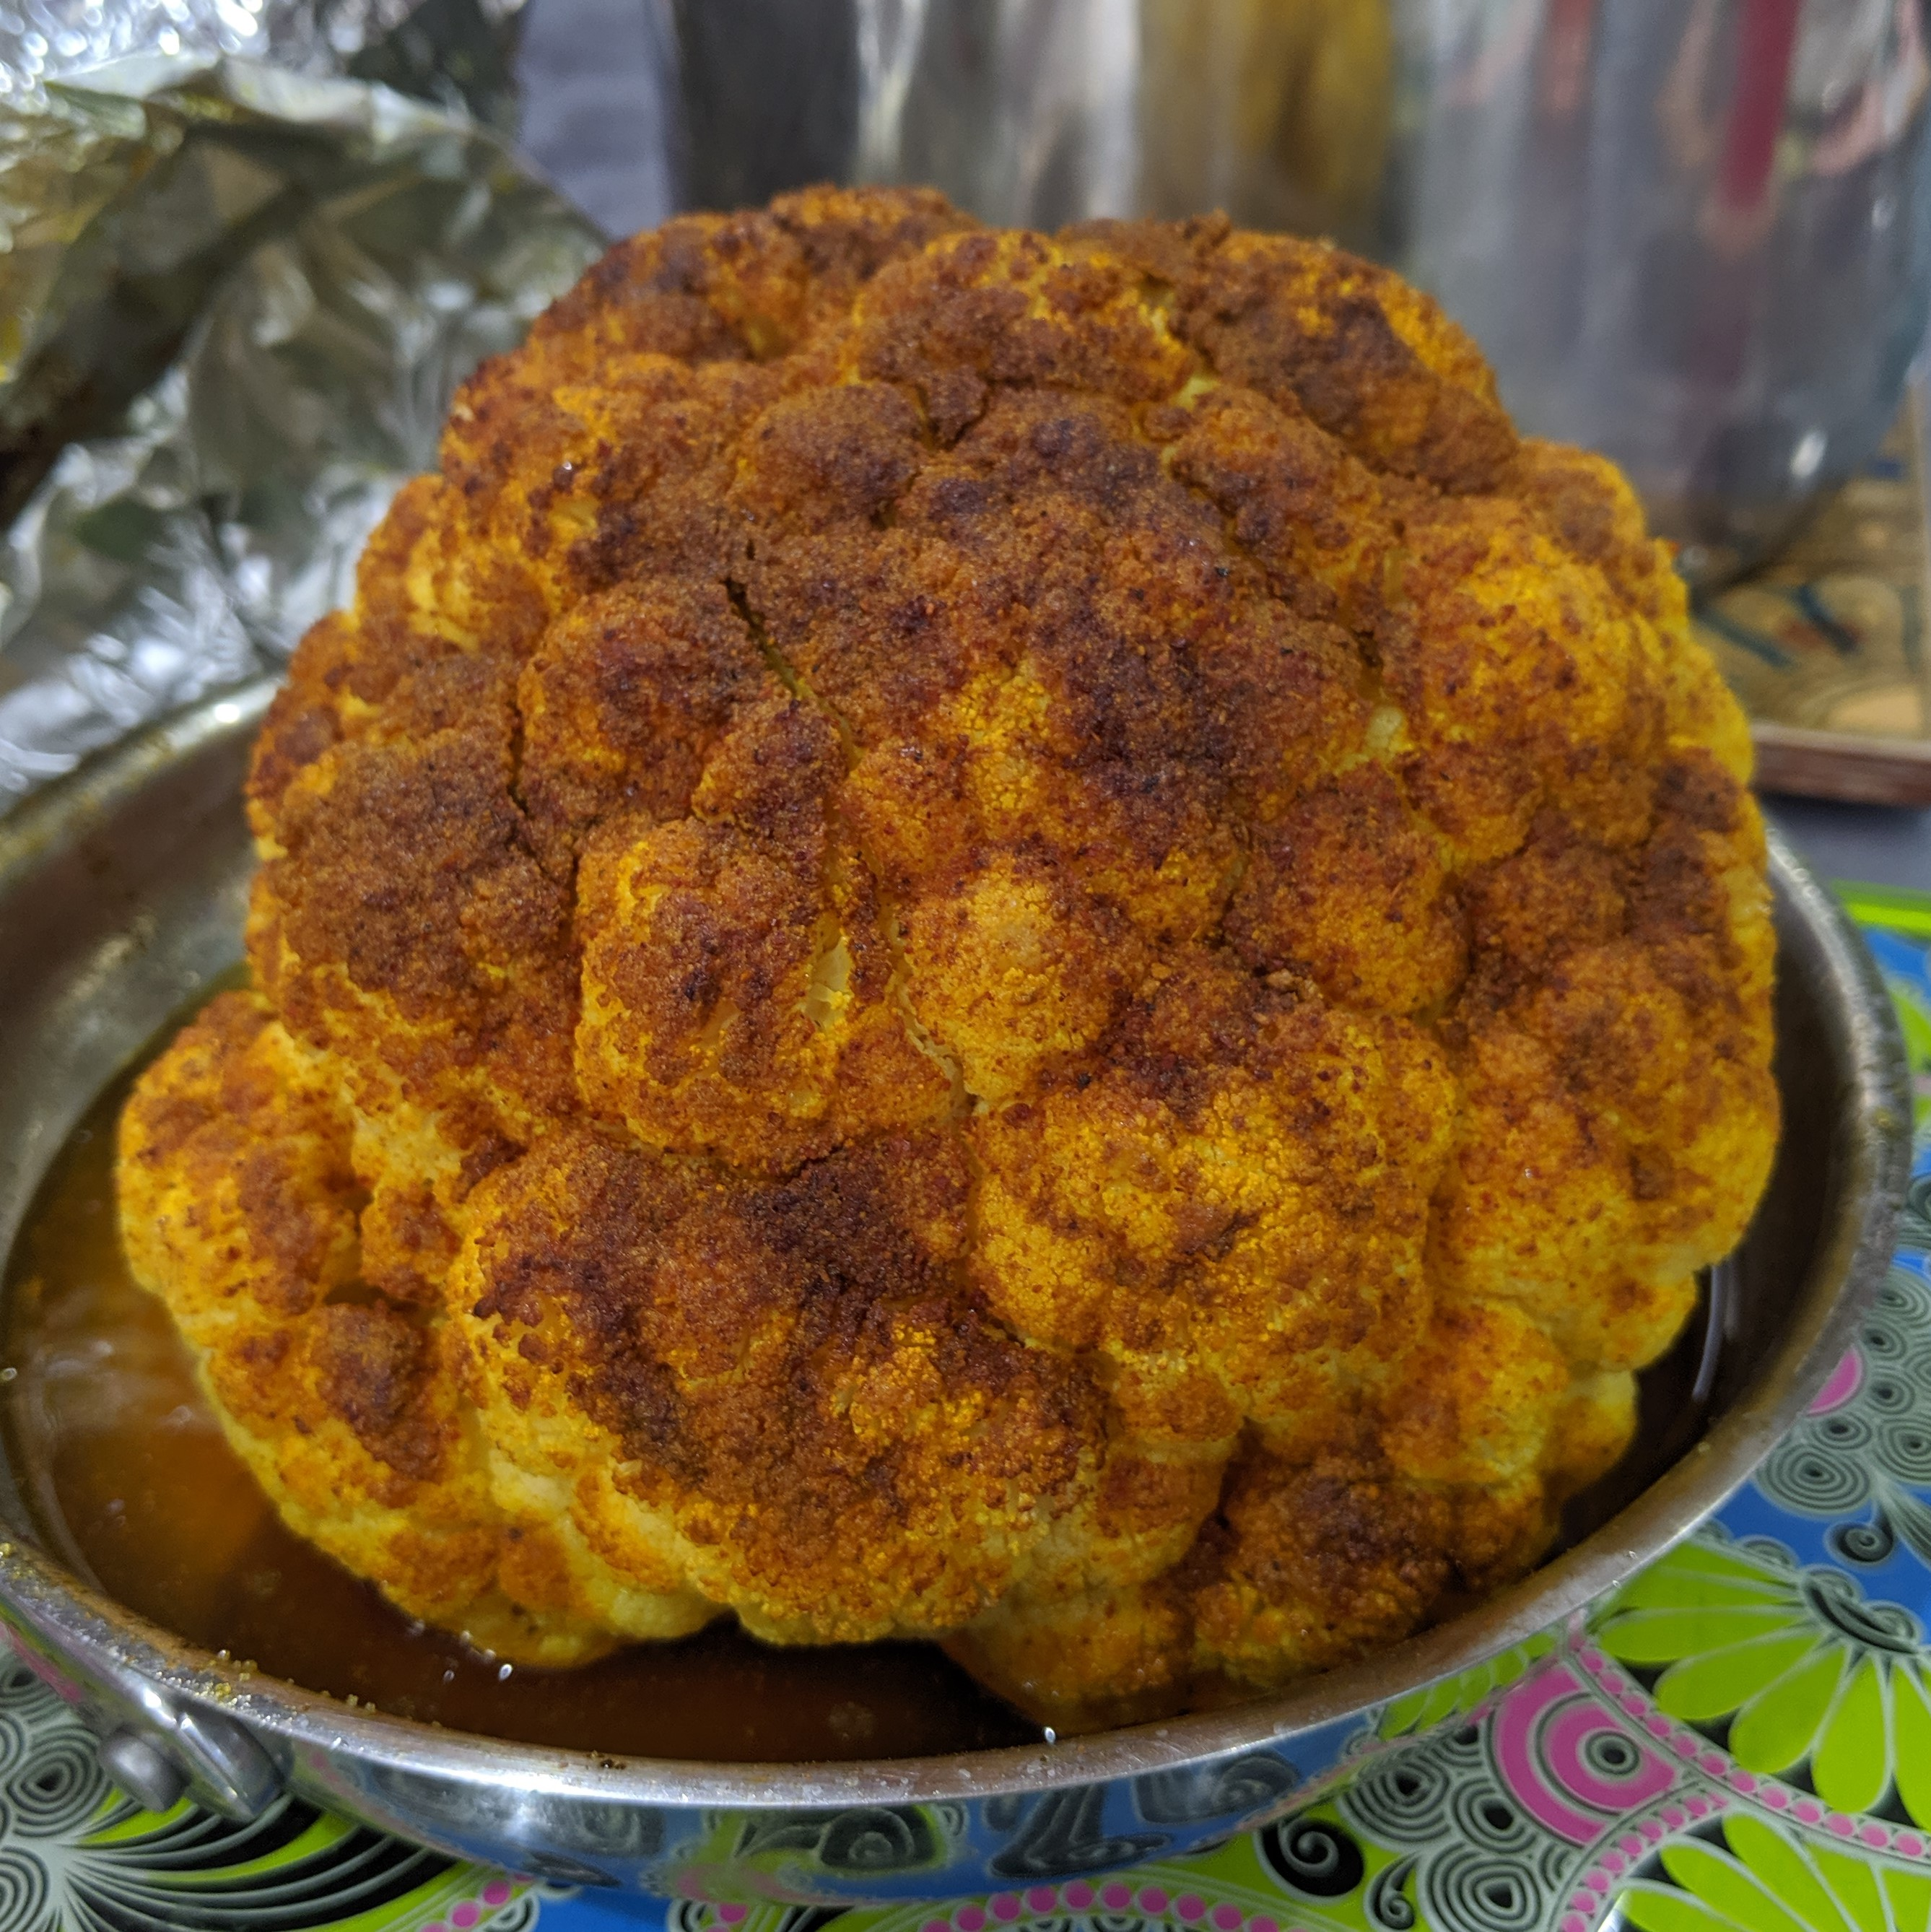
\includegraphics[width=0.15\textwidth]{spicy-whole-roasted-cauliflower}}}\end{floatingfigure}\begin{huge}Spicy Whole Roasted Cauliflower\end{huge}\newline\vspace{-2.5mm}\newline\renewcommand{\arraystretch}{1.1}\begin{tabular*}{\textwidth}{@{\extracolsep{\fill}}lr}A satisfying main dish with a nice kick\\Sunny C\end{tabular*}\newline\vspace{10mm}\newline\begin{huge}Ingredients\end{huge}\\\rule[2.8mm]{\textwidth}{.1pt}\vspace{-3mm}\begin{itemize}\item 1 medium-large head cauliflower\item 3 tbs olive oil\item 1 teas paprika\item $\frac{1}{2}$ teas turmeric\item $\frac{1}{2}$ teas salt\item $\frac{1}{4}$ teas cayenne powder\item 1 cup water\end{itemize}\vspace{7mm}\begin{huge}Directions\end{huge}\\\rule[2.8mm]{\textwidth}{.1pt}\vspace{-3mm}\begin{enumerate}\item Preheat oven to 425\textdegree F. Mix paprika, turmeric, salt, and cayenne in small bowl and set aside.\item Trim leaves from cauliflower and cut stem flat on the bottom.\item Brush cauliflower with olive oil, coating thoroughly. Sprinkle all over with spice mixture.\item Place cauliflower in a small, oven-safe dish and cover completely with foil. Add water to bottom of dish and roast in preheated oven for 1 hour 15 minutes.\item Top with tahini sauce if desired.\end{enumerate}\end{document}